% Options for packages loaded elsewhere
\PassOptionsToPackage{unicode}{hyperref}
\PassOptionsToPackage{hyphens}{url}
\PassOptionsToPackage{dvipsnames,svgnames,x11names}{xcolor}
%
\documentclass[
]{article}
\title{SUPPLEMENTARY MATERIALS for\\
\strut \\
\textbf{Generalized additive models to analyze biomedical non-linear longitudinal data in R:}\\
Beyond repeated measures ANOVA and Linear Mixed Models\\
\strut \\
APPENDIX B: CODE AND FUNCTIONS}
\author{}
\date{\vspace{-2.5em}}

\usepackage{amsmath,amssymb}
\usepackage{lmodern}
\usepackage{iftex}
\ifPDFTeX
  \usepackage[T1]{fontenc}
  \usepackage[utf8]{inputenc}
  \usepackage{textcomp} % provide euro and other symbols
\else % if luatex or xetex
  \usepackage{unicode-math}
  \defaultfontfeatures{Scale=MatchLowercase}
  \defaultfontfeatures[\rmfamily]{Ligatures=TeX,Scale=1}
\fi
% Use upquote if available, for straight quotes in verbatim environments
\IfFileExists{upquote.sty}{\usepackage{upquote}}{}
\IfFileExists{microtype.sty}{% use microtype if available
  \usepackage[]{microtype}
  \UseMicrotypeSet[protrusion]{basicmath} % disable protrusion for tt fonts
}{}
\makeatletter
\@ifundefined{KOMAClassName}{% if non-KOMA class
  \IfFileExists{parskip.sty}{%
    \usepackage{parskip}
  }{% else
    \setlength{\parindent}{0pt}
    \setlength{\parskip}{6pt plus 2pt minus 1pt}}
}{% if KOMA class
  \KOMAoptions{parskip=half}}
\makeatother
\usepackage{xcolor}
\IfFileExists{xurl.sty}{\usepackage{xurl}}{} % add URL line breaks if available
\IfFileExists{bookmark.sty}{\usepackage{bookmark}}{\usepackage{hyperref}}
\hypersetup{
  colorlinks=true,
  linkcolor={Maroon},
  filecolor={Maroon},
  citecolor={Blue},
  urlcolor={blue},
  pdfcreator={LaTeX via pandoc}}
\urlstyle{same} % disable monospaced font for URLs
\usepackage[margin=1in]{geometry}
\usepackage{listings}
\newcommand{\passthrough}[1]{#1}
\lstset{defaultdialect=[5.3]Lua}
\lstset{defaultdialect=[x86masm]Assembler}
\usepackage{longtable,booktabs,array}
\usepackage{calc} % for calculating minipage widths
% Correct order of tables after \paragraph or \subparagraph
\usepackage{etoolbox}
\makeatletter
\patchcmd\longtable{\par}{\if@noskipsec\mbox{}\fi\par}{}{}
\makeatother
% Allow footnotes in longtable head/foot
\IfFileExists{footnotehyper.sty}{\usepackage{footnotehyper}}{\usepackage{footnote}}
\makesavenoteenv{longtable}
\usepackage{graphicx}
\makeatletter
\def\maxwidth{\ifdim\Gin@nat@width>\linewidth\linewidth\else\Gin@nat@width\fi}
\def\maxheight{\ifdim\Gin@nat@height>\textheight\textheight\else\Gin@nat@height\fi}
\makeatother
% Scale images if necessary, so that they will not overflow the page
% margins by default, and it is still possible to overwrite the defaults
% using explicit options in \includegraphics[width, height, ...]{}
\setkeys{Gin}{width=\maxwidth,height=\maxheight,keepaspectratio}
% Set default figure placement to htbp
\makeatletter
\def\fps@figure{htbp}
\makeatother
\setlength{\emergencystretch}{3em} % prevent overfull lines
\providecommand{\tightlist}{%
  \setlength{\itemsep}{0pt}\setlength{\parskip}{0pt}}
\setcounter{secnumdepth}{5}
%\usepackage{lineno}
\usepackage[affil-it,blocks]{authblk}
\usepackage{hyperref}
\usepackage{graphicx}
%\usepackage[nomarkers,figuresonly]{endfloat}
%set a box to put the ORCID logo
\newbox{\myorcidaffilbox}
\sbox{\myorcidaffilbox}{\large
\includegraphics[height=1.7ex]{latex_docs/orcid}}

%add hyperlink to the box
\newcommand{\orcidaffila}[1]{%
  \href{https://orcid.org/0000-0002-6014-4538}{\usebox{\myorcidaffilbox}}}

\newcommand{\orcidaffilb}[1]{%
  \href{https://orcid.org/0000-0002-6135-8191}{\usebox{\myorcidaffilbox}}}

%start sections and page numbers with A
\setcounter{page}{1}
\renewcommand\thesection{B}
\renewcommand\thesubsection{\thesection.\arabic{subsection}}
\renewcommand{\thepage}{B-\arabic{page}}


%command for the package lineno
%\linenumbers

%authors
\author{Ariel I. Mundo \orcidaffila{}}
%\affil{Department of Biomedical Engineering, University of Arkansas, Fayetteville, AR, USA}
\author{John R. Tipton \orcidaffilb{}}
%\affil{Department of Mathematical Sciences, University of Arkansas, Fayetteville, AR, USA}
\author{Timothy J. Muldoon*}
%\affil{Department of Biomedical Engineering, University of Arkansas, Fayetteville, AR, USA}
\affil{tmuldoon@uark.edu}


%theme colors for the code chunks (originally from latex-solarized on GitHub)
%https://github.com/jez/latex-solarized
\usepackage{xcolor}
\definecolor{sbase03}{HTML}{002B36}
\definecolor{sbase02}{HTML}{073642}
\definecolor{sbase01}{HTML}{586E75}
\definecolor{sbase00}{HTML}{657B83}
\definecolor{sbase0}{HTML}{839496}
\definecolor{sbase1}{HTML}{93A1A1}
\definecolor{sbase2}{HTML}{EEE8D5}
\definecolor{sbase3}{HTML}{FDF6E3}
\definecolor{syellow}{HTML}{B58900}
\definecolor{sorange}{HTML}{CB4B16}
\definecolor{sred}{HTML}{DC322F}
\definecolor{smagenta}{HTML}{D33682}
\definecolor{sviolet}{HTML}{6C71C4}
\definecolor{sblue}{HTML}{268BD2}
\definecolor{scyan}{HTML}{2AA198}
\definecolor{sgreen}{HTML}{859900}
%command to set parameter(s) in package listings
\lstset{
    % How/what to match
    sensitive=true,
    % Border (above and below)
    frame=lines,
    % Extra margin on line (align with paragraph)
    xleftmargin=\parindent,
    % Put extra space under caption
    belowcaptionskip=1\baselineskip,
    % Colors
    backgroundcolor=\color{sbase3},
    basicstyle=\color{sbase00}\ttfamily,
    keywordstyle=\color{scyan},
    commentstyle=\color{sbase1},
    stringstyle=\color{sblue},
    numberstyle=\color{sviolet},
    identifierstyle=\color{sbase00},
    % Break long lines into multiple lines?
    breaklines=true,
    % Show a character for spaces?
    showstringspaces=false,
    tabsize=2
}


%\lstset{
%  breaklines=true,
%  stringstyle=\ttfamily,
%  backgroundcolor=\color{gray}
%}
\usepackage{placeins}
\usepackage{subfig}
\usepackage{breqn}
\usepackage[font={small}]{caption}
\usepackage{float}
\ifLuaTeX
  \usepackage{selnolig}  % disable illegal ligatures
\fi

\begin{document}
\maketitle

\newpage

\counterwithin{figure}{section}

This appendix shows the code for the functions used through the main manuscript, which can be found in the \emph{scripts} folder in the GitHub repository. We provide a brief explanation of the purpose of each function.

\hypertarget{setup}{%
\subsection{Setup}\label{setup}}

First, we load all required libraries and set seed.

\begin{lstlisting}[language=R]
library(patchwork)
library(tidyverse)
library(mvnfast)
library(nlme)
library(mgcv)
library(gratia)
library(here)
library(scico)
set.seed(2021) #set seed for reproducibility

#alpha for ribbon in the smooth plots
al<-0.8

thm1<-scale_fill_scico_d(palette="tokyo",begin=0.3, end=0.8, direction = -1, aesthetics = c("colour","fill"))
\end{lstlisting}

\hypertarget{linear-and-quadratic-longitudinal-trends}{%
\subsection{Linear and quadratic longitudinal trends}\label{linear-and-quadratic-longitudinal-trends}}

\hypertarget{function-for-linear-and-quadratic-trends-rm-anova-and-lmem-fits}{%
\subsubsection{Function for linear and quadratic trends, rm-ANOVA and LMEM fits}\label{function-for-linear-and-quadratic-trends-rm-anova-and-lmem-fits}}

The first function is \passthrough{\lstinline!example.R!}, which allows to simulate linear and quadratic data in the same manner as in Section 3.5 in the main manuscript and estimates rm-ANOVA and LMEM with interaction to the data. The error for each simulated trend can be correlated or uncorrelated

\begin{lstlisting}[language=R]
##########Section for calculations###########

## Example with linear response

#This function simulates data using a linear or quadratic mean response and each with correlated
#or uncorrelated errors. Each group has a different slope/concavity.
example <- function(n_time = 6, #number of time points
                    fun_type = "linear", #type of response
                    error_type = "correlated") {
  
  if (!(fun_type %in% c("linear", "quadratic")))
    stop('fun_type must be either "linear", or "quadratic"')
  if (!(error_type %in% c("correlated", "independent")))
    stop('fun_type must be either "correlated", or "independent"')
  
  
  x <- seq(1,6, length.out = n_time)
  
  #Create mean response matrix: linear or quadratic
  mu <- matrix(0, length(x), 2)
  # linear response
  if (fun_type == "linear") {
    mu[, 1] <- - (0.25*x)+2  
    mu[, 2] <- 0.25*x+2
  } else {
    # quadratic response (non-linear)
    
    mu[, 1] <-  -(0.25 * x^2) +1.5*x-1.25
    mu[, 2] <- (0.25 * x^2) -1.5*x+1.25
  }
  
 
  #create an array where individual observations per each time point for each group are to be stored. Currently using 10 observations per timepoint
  y <- array(0, dim = c(length(x), 2, 10))
  
  #Create array to store the "errors" for each group at each timepoint. The "errors" are the 
  #between-group variability in the response.
  errors <- array(0, dim = c(length(x), 2, 10))
  #create an array where 10 observations per each time point for each group are to be stored
  
  #The following loops create independent or correlated responses. To each value of mu (mean response per group) a randomly generated error (correlated or uncorrelated) is added and thus the individual response is created.
  if (error_type == "independent") {
    ## independent errors
    for (i in 1:2) {
      for (j in 1:10) {
        errors[, i, j] <- rnorm(6, 0, 0.25)
        y[, i, j] <- mu[, i] + errors[, i, j]
      }
    }
  } else {
    for (i in 1:2) {     # number of treatments
      for (j in 1:10) {  # number of subjects
        # compound symmetry errors: variance covariance matrix
        errors[, i, j] <- rmvn(1, rep(0, length(x)), 0.1 * diag(6) + 0.25 * matrix(1, 6, 6))
        y[, i, j] <- mu[, i] + errors[, i, j]
      }
    }
  }    
  
  
  ## subject random effects
  
  ## visualizing the difference between independent errors and compound symmetry
  ## why do we need to account for this -- overly confident inference
  
#labeling y and errors  
  dimnames(y) <- list(time = x, 
                      treatment = 1:2, 
                      subject = 1:10)

  dimnames(errors) <- list(time = x, 
                           treatment = 1:2, 
                           subject = 1:10)
  
  #labeling the mean response
  dimnames(mu) <- list(time = x, 
                       treatment = 1:2)
  
  #convert y, mu and errors to  dataframes with time, treatment and subject columns
  dat <- as.data.frame.table(y, 
                             responseName = "y")
  dat_errors <- as.data.frame.table(errors, 
                                    responseName = "errors")
  dat_mu <- as.data.frame.table(mu, 
                                responseName = "mu")
  
  #join the dataframes to show mean response and errors per subject
  dat <- left_join(dat, dat_errors, 
                   by = c("time", "treatment", "subject"))
  dat <- left_join(dat, dat_mu, 
                   by = c("time", "treatment"))
  #add time
  dat$time <- as.numeric(as.character(dat$time))
  #label subjects per group
  dat <- dat %>%
    mutate(subject = factor(paste(subject, 
                                  treatment, 
                                  sep = "-")))
  
  
  ## repeated measures ANOVA 
  
  fit_anova <- lm(y ~ time + treatment + time * treatment, data = dat)
  
#LMEM: time and treatment interaction model, compound symmetry 
  fit_lme <- lme(y ~ treatment + time + treatment:time,
                 data = dat,
                 random = ~ 1 | subject,
                 correlation = corCompSymm(form = ~ 1 | subject)
  )
  
  #create a prediction frame where the model can be used for plotting purposes
  pred_dat <- expand.grid(
    treatment = factor(1:2), 
    time = unique(dat$time)
  )
  
  #add model predictions to the dataframe that has the simulated data
  dat$pred_anova <- predict(fit_anova)
  dat$pred_lmem <- predict(fit_lme)

  #return everything in a list
  return(list(
    dat = dat,
    pred_dat = pred_dat,
    fit_anova=fit_anova,
    fit_lme = fit_lme
  ))
}
\end{lstlisting}

\hypertarget{a-composite-plot-for-the-trends}{%
\subsubsection{A composite plot for the trends}\label{a-composite-plot-for-the-trends}}

Function \passthrough{\lstinline!plot\_example.R!} uses the output of \passthrough{\lstinline!example.R!} to show the fit of a rm-ANOVA and a LMEM. It can be used to show an expanded version of Figure 1 in the main manuscript, presenting simulated data with correlated and uncorrelated errors and the correspoding rm-ANOVA and LMEM fits, which we do in the next subsection.

\begin{lstlisting}[language=R]
## This function plots the rm-ANOVA and LMEM for the data simulated in example.R
plot_example <- function(sim_dat) {
    # Plot the simulated data (scatterplot)
    p1 <- sim_dat$dat %>%
        ggplot(aes(x = time,
                   y = y,
                   group = treatment,
                   color = treatment)
        ) +
        geom_point(alpha=0.5,
                   show.legend=FALSE) +
        labs(y='response')+
        geom_line(aes(x = time,
                      y = mu,
                      color = treatment),
                  size=3,
                  show.legend=FALSE) +
        theme_classic() +
        theme(plot.title = element_text(size = 20,
                                        face = "bold"),
              text=element_text(size=20))+
        thm1

    #plot the model predictions for rm-ANOVA
    p2 <- ggplot(sim_dat$dat,
                 aes(x = time,
                     y = y,
                     color = treatment)) +
        geom_point(alpha=0.5,
                   show.legend=FALSE)+
        labs(y='response')+
        geom_line(aes(y = predict(sim_dat$fit_anova),
                      group = subject, size = "Subjects"),
                  show.legend = FALSE) +
        geom_line(data = sim_dat$pred_dat,
                  aes(y = predict(sim_dat$fit_anova,
                                  level = 0,
                                  newdata = sim_dat$pred_dat),
                      size = "Population"),
                  show.legend=FALSE) +
        guides(color = guide_legend(override.aes = list(size = 2)))+
        scale_size_manual(name = "Predictions",
                          values=c("Subjects" = 0.5, "Population" = 3)) +
        theme_classic() +
        theme(plot.title = element_text(size = 20,
                                        face = "bold"),
              text=element_text(size=20))+
        thm1

    #plot the model predictions for LMEM
    p4 <- ggplot(sim_dat$dat,
                 aes(x = time,
                     y = y,
                     color = treatment)) +
        geom_point(alpha=0.5)+
        labs(y='response')+
        geom_line(aes(y = predict(sim_dat$fit_lme),
                      group = subject, size = "Subjects")) +
        geom_line(data = sim_dat$pred_dat,
                  aes(y = predict(sim_dat$fit_lme,
                                  level = 0,
                                  newdata = sim_dat$pred_dat),
                      size = "Population")) +
        guides(color = guide_legend(override.aes = list(size = 2)))+
        scale_size_manual(name = "Predictions",
                          values=c("Subjects" = 0.5, "Population" = 3)) +
        theme_classic() +
        theme(plot.title = element_text(size = 20,
                                        face = "bold"),
              text=element_text(size=20))+
        thm1

    return((p1+p3+p2+p4+p5)+plot_layout(nrow=1)+plot_annotation(tag_levels = 'A'))

}
\end{lstlisting}

\hypertarget{plotting-rm-anova-and-lmem-fits-for-linear-and-quadratic-trends-in-data}{%
\subsubsection{Plotting rm-ANOVA and LMEM fits for linear and quadratic trends in data}\label{plotting-rm-anova-and-lmem-fits-for-linear-and-quadratic-trends-in-data}}

In this subsection, we use \passthrough{\lstinline!example.R!} and a modified version \passthrough{\lstinline!plot\_example.R!} (\passthrough{\lstinline!plot\_example\_Appendix.R!}) to create an expanded version of Figure 1 on the main manuscript. The only difference between \passthrough{\lstinline!plot\_example.R!} and \passthrough{\lstinline!plot\_example\_Appendix.R!} is the inclusion of a \passthrough{\lstinline!ggplot2!} object (\passthrough{\lstinline!p3!}) that allows to plot the simulated errors.

Figure \ref{fig:linear-cases-Appendix} show in panels A and D the simulated mean responses and individual data points. Panels C and G show a visual interpretation of ``correlation'' in the responses: In panel C, subjects that have a value of the random error \(\varepsilon\) either above or below the mean group response are more likely to have other observations that follow the same trajectory, thereby demonstrating correlation in the response. In panel G,because the errors are independent, there is no expectation that responses are likely to follow a similar pattern. Panels D and H show the predictions from the rm-ANOVA model.

\hypertarget{fits-for-linear-trends}{%
\paragraph{Fits for linear trends}\label{fits-for-linear-trends}}

The chunk below calls both \passthrough{\lstinline!example.R!} and \passthrough{\lstinline!plot\_example\_Appendix.R!} to simulate data and create the composite plots.

\begin{lstlisting}[language=R]
source(here::here("Manuscripts/Manuscript_by_chapters-SIM_Revisions_final/scripts","example.R"))
source(here::here("Manuscripts/Manuscript_by_chapters-SIM_Revisions_final/scripts","plot_example_Appendix.R"))

A1<-plot_example_Appendix(example(fun_type = "linear", error_type = "correlated")) 

B1<-plot_example_Appendix(example(fun_type = "linear", error_type = "independent")) 
  
C1<-plot_example_Appendix(example(fun_type = "quadratic", error_type = "correlated")) 
  
D1<-plot_example_Appendix(example(fun_type = "quadratic", error_type = "independent")) 
\end{lstlisting}



\begin{figure}

{\centering 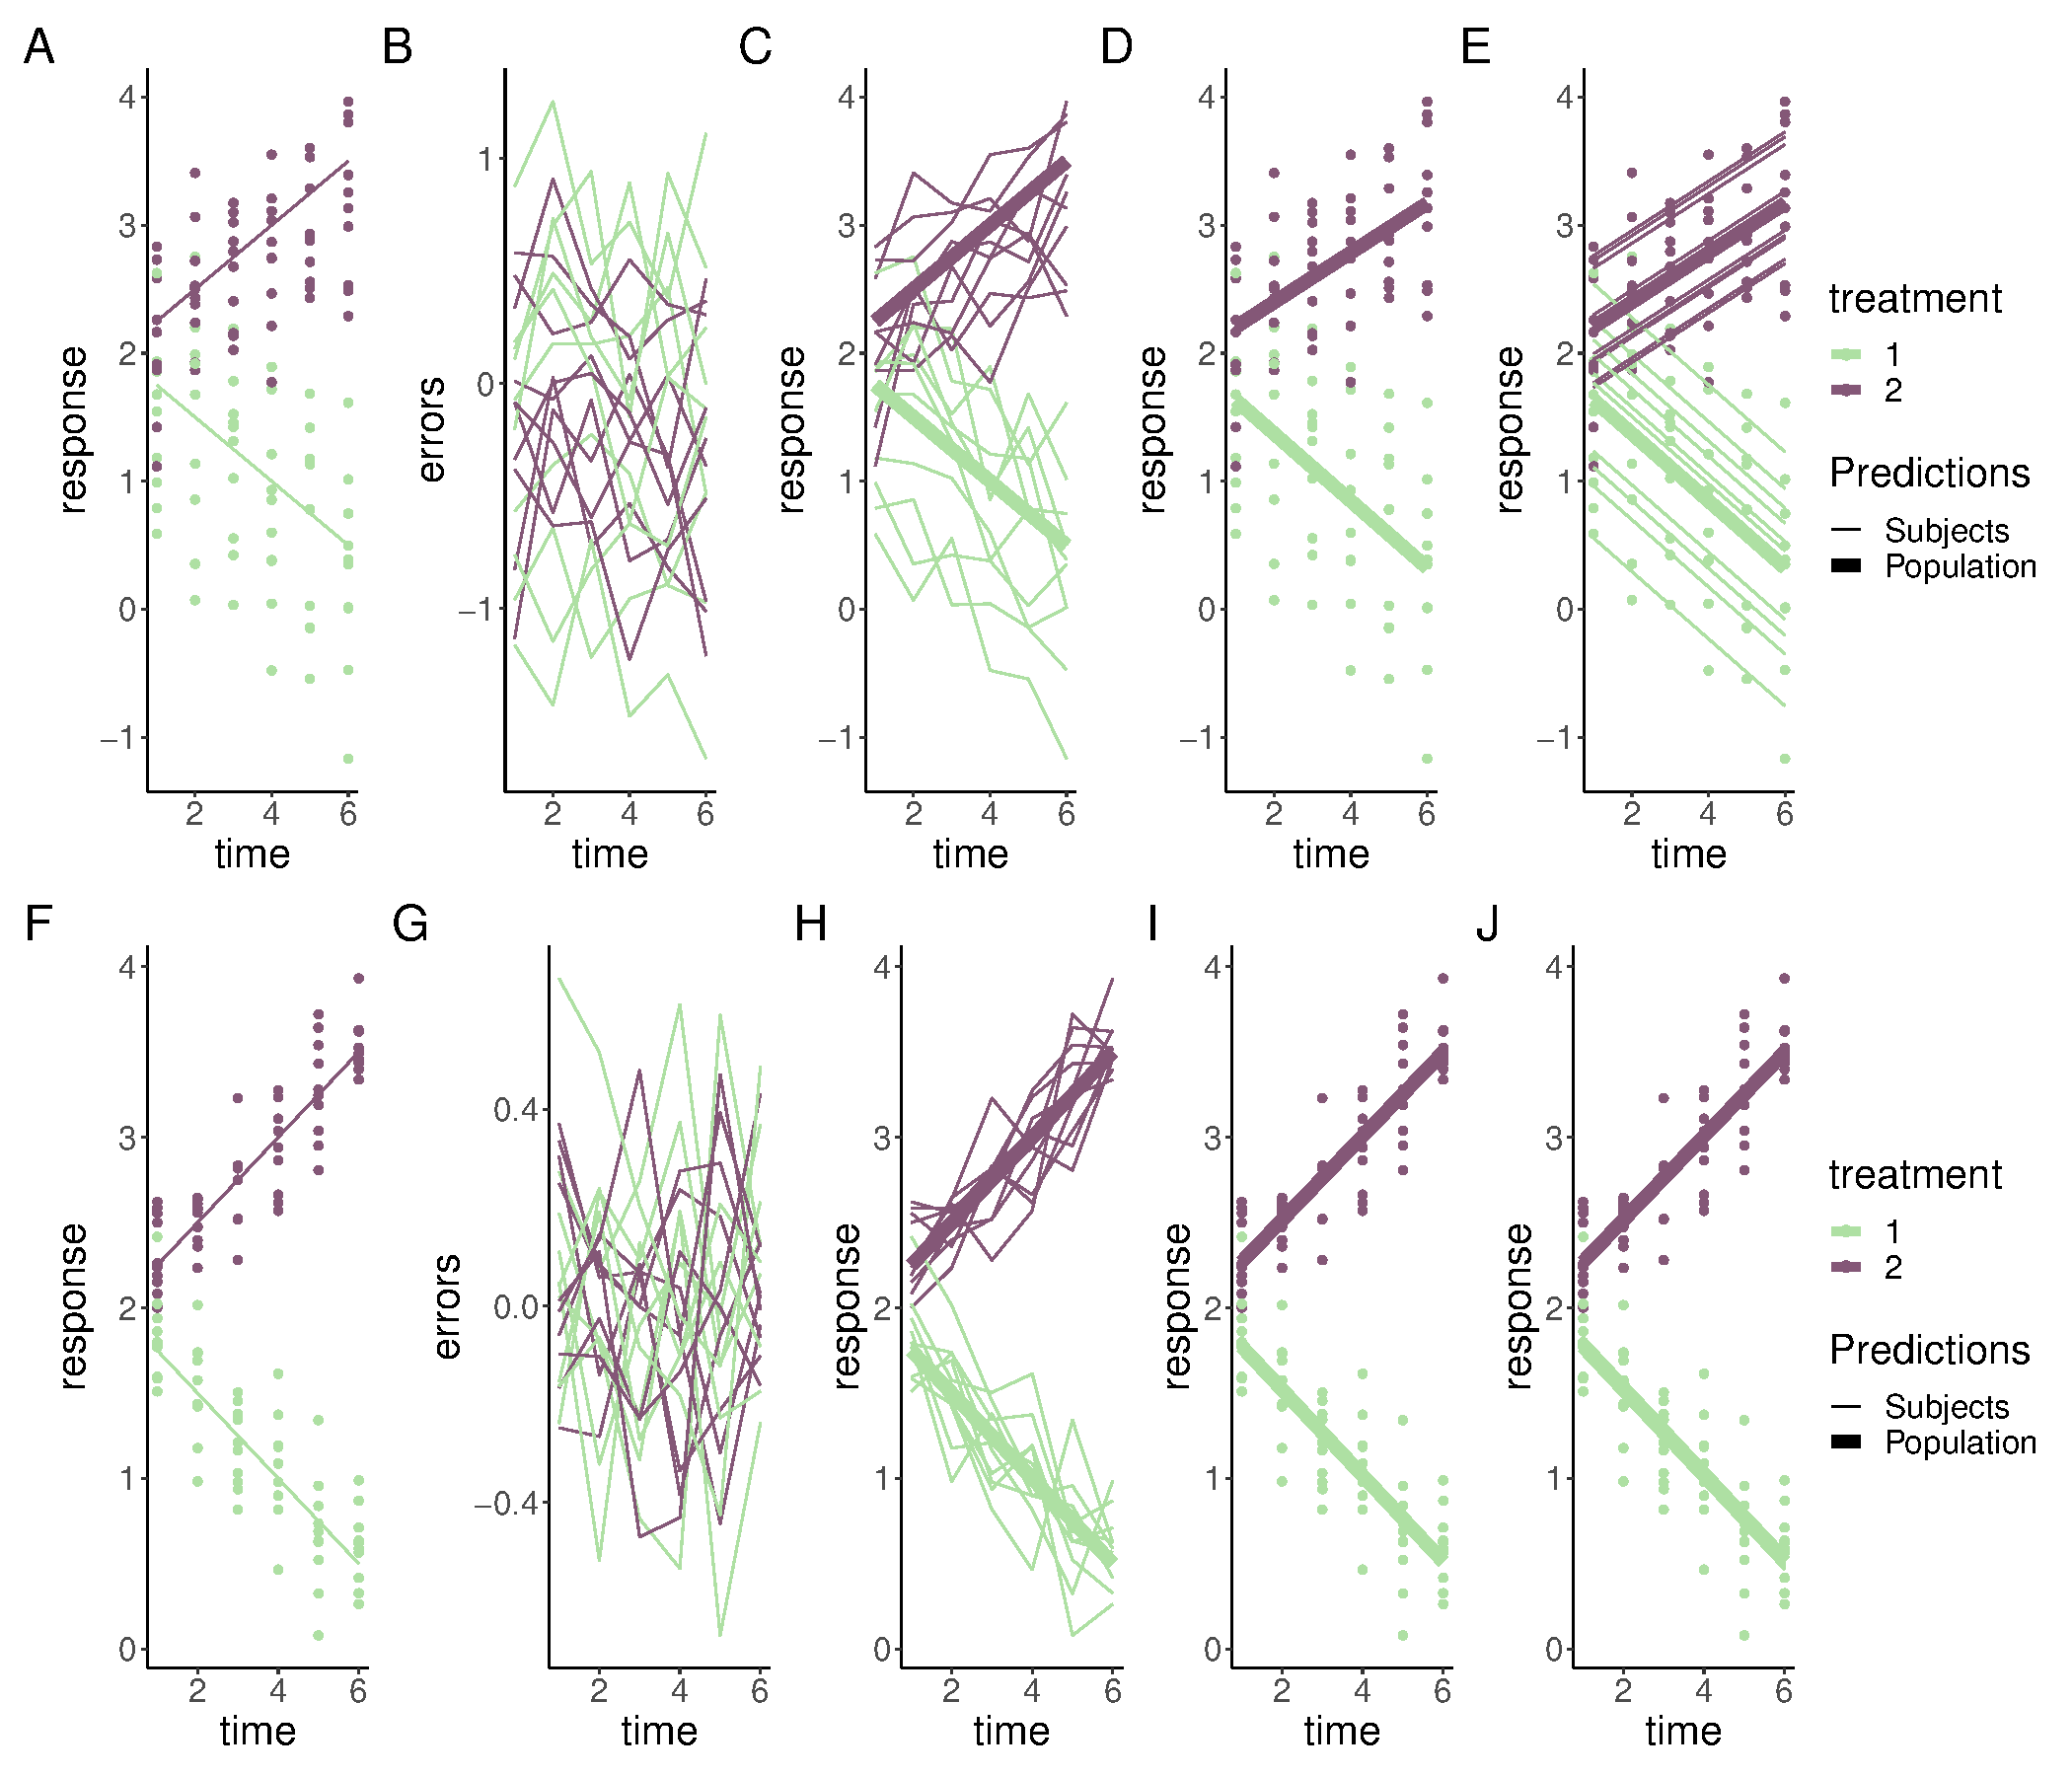
\includegraphics[width=1\linewidth]{Appendix_B_files/figure-latex/linear-cases-Appendix-1} 

}

\caption{Simulated linear responses from two groups with correlated (top row) or independent (bottom row) errors using a rm-ANOVA model and a LMEM. A, F:Simulated data with known mean response and individual responses (points) showing the dispersion of the data. B,G: Generated errors showing the difference in the behavior of correlated and independent errors. C,H: Simulated data with thin lines representing individual trajectories. D,I: Estimations from the rm-ANOVA model for the mean group response. E, J: Estimations from the LMEM for the mean group response and individual responses (thin lines). In all panels, thick lines are the predicted mean response per group, thin lines are the random effects for each subject and points represent the original raw data. Both rm-ANOVA and the LMEM are able to capture the trend of the data.}\label{fig:linear-cases-Appendix}
\end{figure}

\hypertarget{fits-for-quadratic-trends}{%
\paragraph{Fits for quadratic trends}\label{fits-for-quadratic-trends}}

For the quadratic response case, Figure \ref{fig:quadratic-cases-Appendix} shows the simulated responses using compound symmetry and independent errors.



\begin{figure}

{\centering 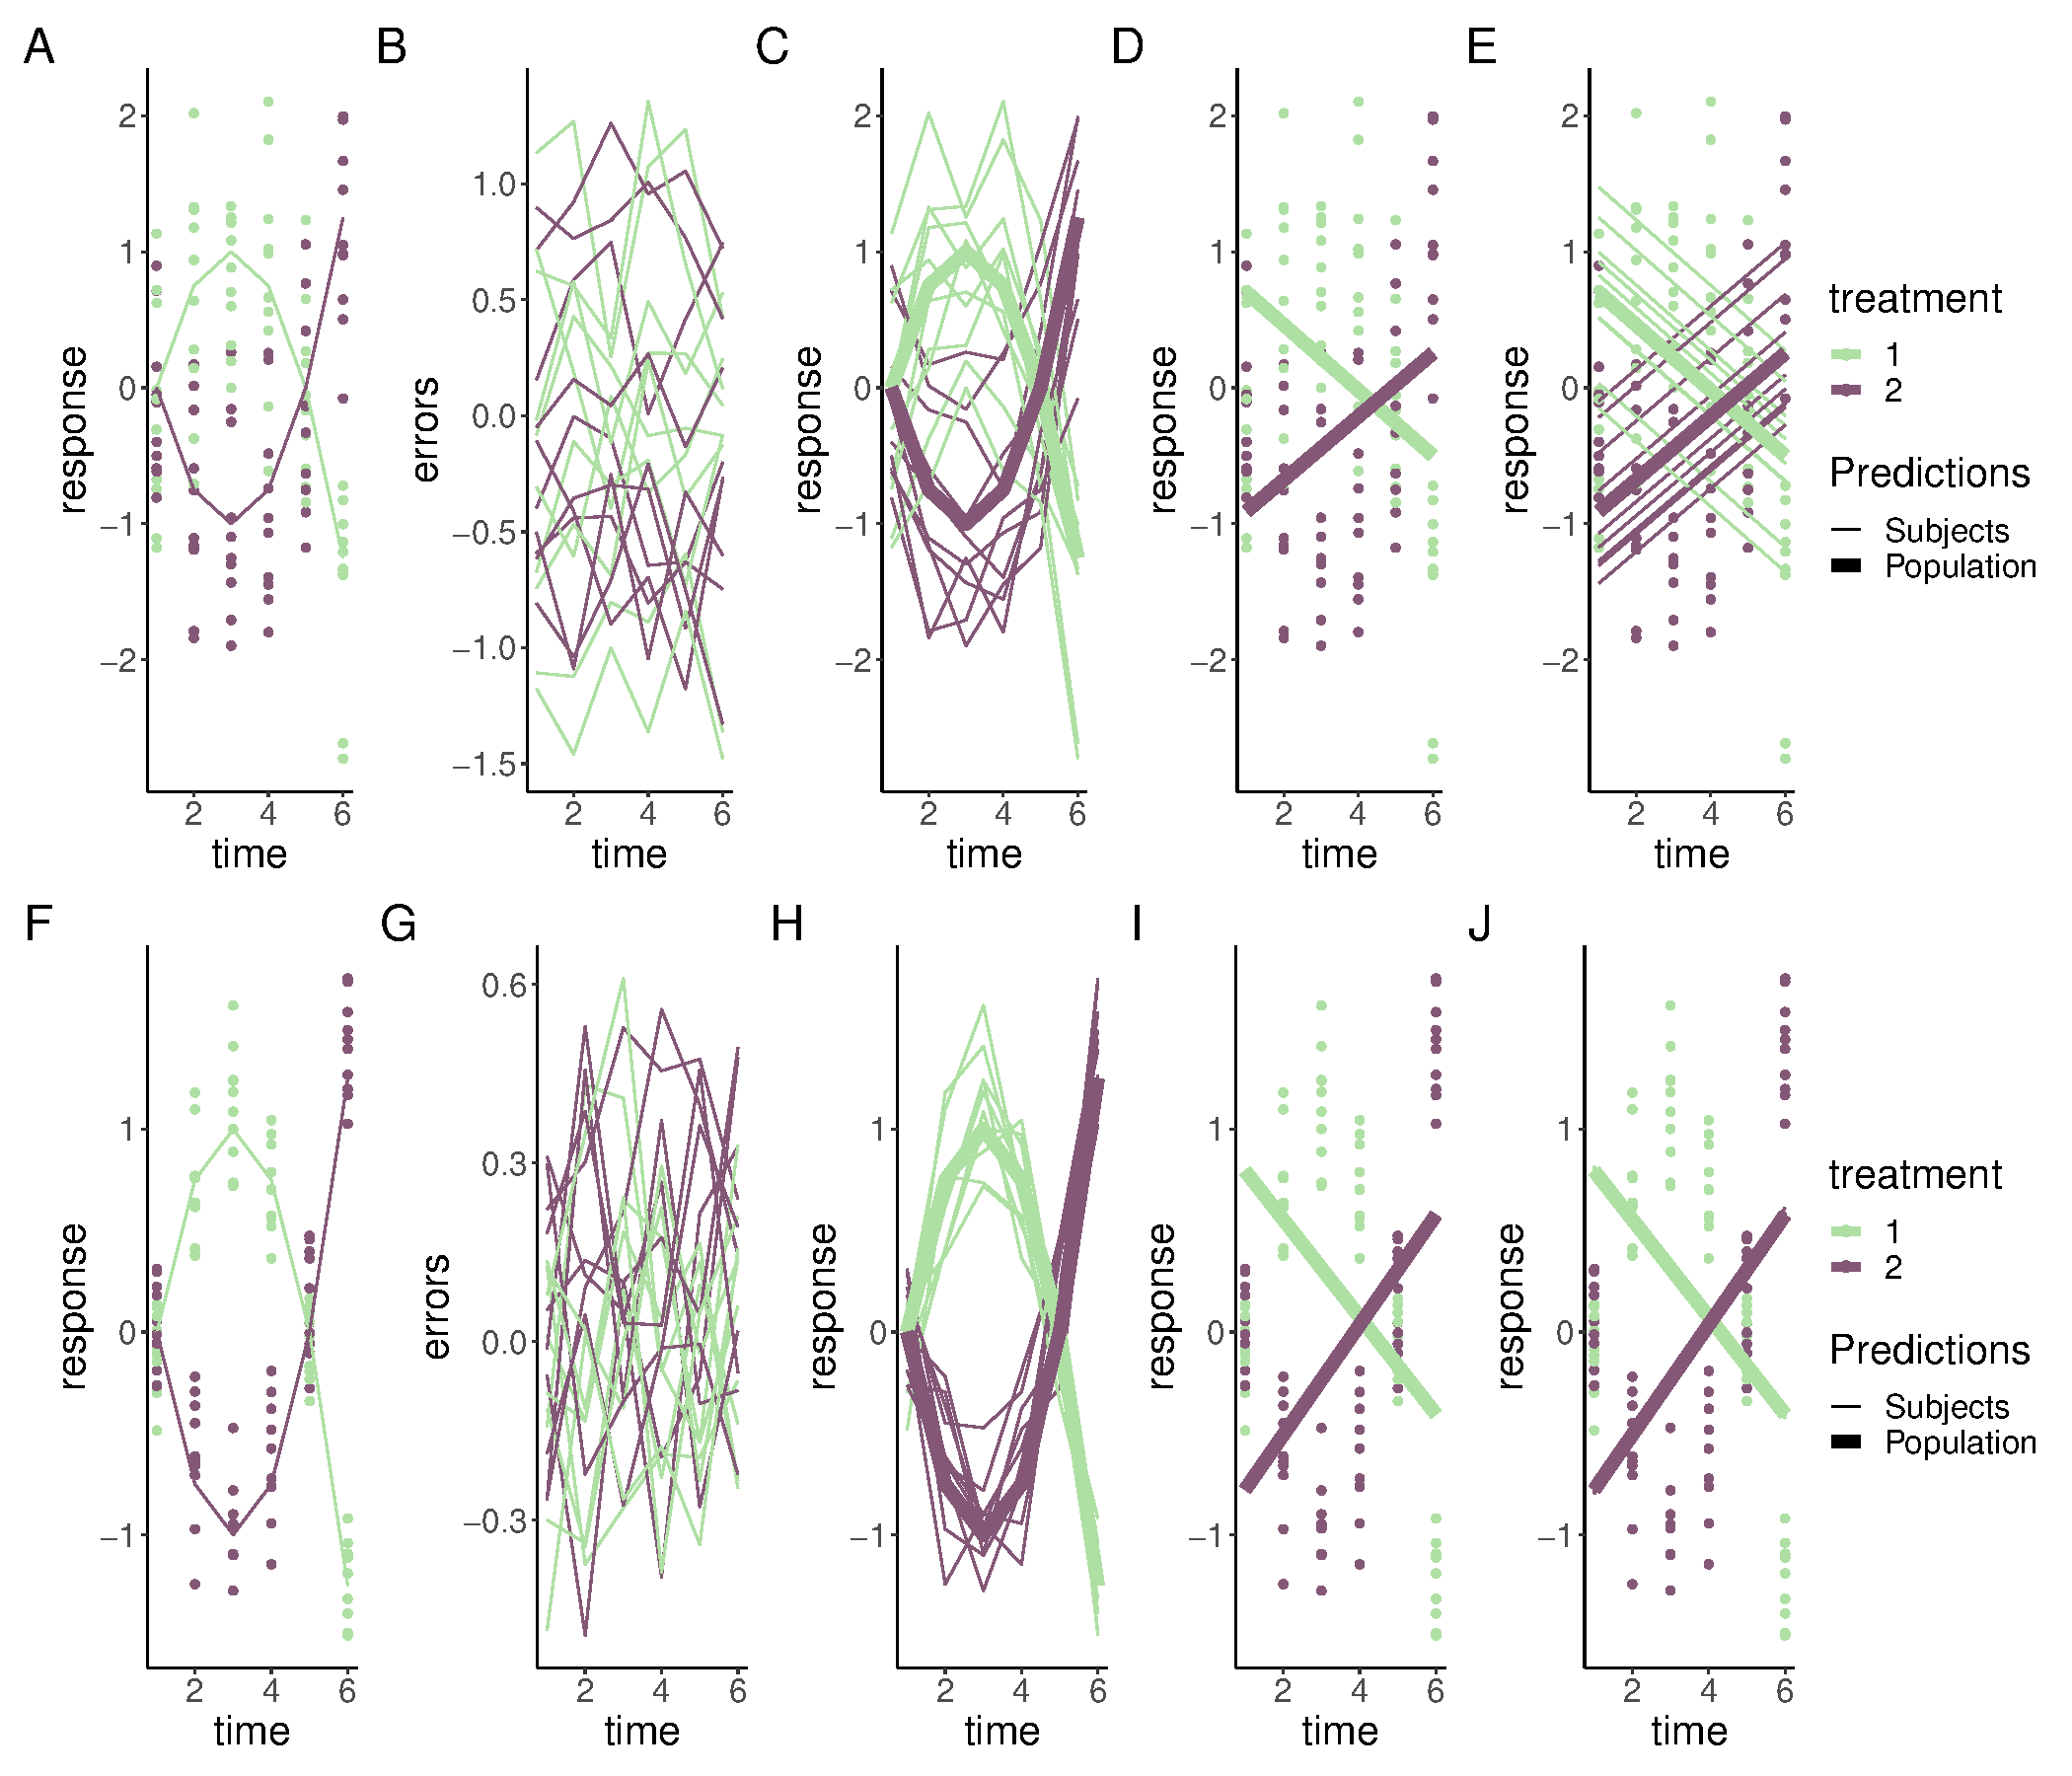
\includegraphics[width=1\linewidth]{Appendix_B_files/figure-latex/quadratic-cases-Appendix-1} 

}

\caption{Simulated quadratic responses from two groups with correlated (top row) or independent (bottom row) errors using a rm-ANOVA model and a LMEM. A, F:Simulated data with known mean response and individual responses (points) showing the dispersion of the data. B,G: Generated errors showing the difference in the behavior of correlated and independent errors. C,H: Simulated data with thin lines representing individual trajectories. D,I: Estimations from the rm-ANOVA model for the mean group response. E, J: Estimations from the LMEM for the mean group response and individual responses (thin lines). In all panels, thick lines are the predicted mean response per group, thin lines are the random effects for each subject and points represent the original raw data. Both rm-ANOVA and the LMEM are not able to capture the changes in each group over time.}\label{fig:quadratic-cases-Appendix}
\end{figure}

\end{document}
